\documentclass[conference]{IEEEtran}

\usepackage{amsmath,amssymb}
\usepackage{algorithm}
\usepackage{algorithmic}
\usepackage{array}
\usepackage{balance}
\usepackage{booktabs}
\usepackage{graphicx}
\usepackage{microtype}
\usepackage{multirow}
\usepackage{pifont}
\usepackage[table]{xcolor}
\usepackage{xurl}
\usepackage{tikz}
\usetikzlibrary{arrows.meta,backgrounds,calc,fit,positioning,shapes.geometric}
\usepackage[hidelinks,hypertexnames=false]{hyperref}
\vfuzz=2pt

\newcommand{\system}{TokenPowerAgent}
\newcommand{\sandbox}{TokenPowerSandbox}
\newcommand{\bench}{TokenPowerBench}
\newcommand{\ipig}{IPIG}
\newcommand{\cmark}{\textcolor{tpTealDark}{\ding{51}}}
\newcommand{\pmark}{\textcolor{tpGoldDark}{\raisebox{0.1ex}{\scriptsize$\triangle$}}}
\newcommand{\xmark}{\textcolor{tpGray}{\ding{55}}}
\newcommand{\draftvalue}[1]{\textcolor{tpDraft}{\textbf{[#1]}}}

\definecolor{tpTeal}{HTML}{4EA995}
\definecolor{tpTealDark}{HTML}{256F63}
\definecolor{tpTealLight}{HTML}{DDF1EB}
\definecolor{tpRose}{HTML}{D85F7C}
\definecolor{tpRoseDark}{HTML}{8E3650}
\definecolor{tpRoseLight}{HTML}{F7DCE4}
\definecolor{tpGold}{HTML}{D8A945}
\definecolor{tpGoldDark}{HTML}{8A641D}
\definecolor{tpGoldLight}{HTML}{F8EDCD}
\definecolor{tpBlue}{HTML}{4E91AE}
\definecolor{tpBlueDark}{HTML}{285E75}
\definecolor{tpBlueLight}{HTML}{DDEEF5}
\definecolor{tpGray}{HTML}{6D7478}
\definecolor{tpGrayLight}{HTML}{EDF0F1}
\definecolor{tpDraft}{HTML}{7B6B52}

% Two sealed H100/Qwen2.5-7B holdouts generated on 2026-08-04.
% The same frozen v2 model was used for both; no refit occurred between them.
\newcommand{\AnchorRepeats}{3}
\newcommand{\DevelopmentWorkloads}{6}
\newcommand{\DevelopmentMeasurements}{18}
\newcommand{\HoldoutWorkloads}{8}
\newcommand{\HoldoutMeasurements}{24}
\newcommand{\ConfirmationWorkloads}{9}
\newcommand{\ConfirmationMeasurements}{27}
\newcommand{\BlindWorkloads}{17}
\newcommand{\BlindMeasurements}{51}
\newcommand{\MeasuredRunsExcludingAnchors}{69}

\newcommand{\BaseEnergyMAPE}{63.01\%}
\newcommand{\CalibratedEnergyMAPE}{6.23\%}
\newcommand{\EnergyMAPEReduction}{90.1\%}
\newcommand{\EnergyMedianAPE}{4.96\%}
\newcommand{\EnergyMaxAPE}{13.84\%}
\newcommand{\EnergySpearman}{0.976}
\newcommand{\EnergyPairwise}{27/28}
\newcommand{\EnergyPairwisePct}{96.4\%}

\newcommand{\BaseThroughputMAPE}{23.93\%}
\newcommand{\CalibratedThroughputMAPE}{10.53\%}
\newcommand{\ThroughputSpearman}{0.976}
\newcommand{\ThroughputPairwise}{27/28}
\newcommand{\BaseTTFTMAPE}{73.44\%}
\newcommand{\CalibratedTTFTMAPE}{32.67\%}
\newcommand{\TTFTSpearman}{0.952}
\newcommand{\TTFTPairwise}{26/28}
\newcommand{\BaseTPOTMAPE}{34.29\%}
\newcommand{\CalibratedTPOTMAPE}{7.99\%}
\newcommand{\TPOTSpearman}{0.929}
\newcommand{\TPOTPairwise}{25/28}

\newcommand{\DevelopmentLOOEnergyMAPE}{10.11\%}
\newcommand{\EnergyRepeatCV}{0.78\%}
\newcommand{\ThroughputRepeatCV}{0.20\%}
\newcommand{\TPOTRepeatCV}{0.11\%}
\newcommand{\TTFTRepeatCV}{1.74\%}
\newcommand{\PowerMAPE}{8.10\%}
\newcommand{\DurationMAPE}{8.16\%}
\newcommand{\DiagnosticCoverage}{31/32}
\newcommand{\HoldoutGPUHours}{0.144}
\newcommand{\DevelopmentAndHoldoutGPUHours}{0.259}
\newcommand{\TTFTWorstAPE}{138.8\%}

\newcommand{\ConfirmationEnergyMAPE}{7.35\%}
\newcommand{\ConfirmationEnergyMedianAPE}{8.43\%}
\newcommand{\ConfirmationEnergyMaxAPE}{10.93\%}
\newcommand{\ConfirmationEnergySpearman}{0.933}
\newcommand{\ConfirmationEnergyPairwise}{33/36}
\newcommand{\ConfirmationEnergyPairwisePct}{91.7\%}
\newcommand{\ConfirmationThroughputMAPE}{11.31\%}
\newcommand{\ConfirmationTPOTMAPE}{9.03\%}
\newcommand{\ConfirmationTTFTMAPE}{46.29\%}
\newcommand{\ConfirmationEnergyRepeatCV}{0.68\%}
\newcommand{\ConfirmationGPUHours}{0.145}
\newcommand{\TotalCampaignGPUHours}{0.404}

\newcommand{\KOneEnergyMAPE}{5.78\%}
\newcommand{\KOneThroughputMAPE}{24.02\%}
\newcommand{\KOneTPOTMAPE}{18.25\%}
\newcommand{\KOneTTFTMAPE}{79.27\%}
\newcommand{\KTwoEnergyMAPE}{9.15\%}
\newcommand{\KTwoThroughputMAPE}{7.89\%}
\newcommand{\KTwoTPOTMAPE}{6.90\%}
\newcommand{\KTwoTTFTMAPE}{50.34\%}
\newcommand{\KFourEnergyMAPE}{7.12\%}
\newcommand{\KFourThroughputMAPE}{2.01\%}
\newcommand{\KFourTPOTMAPE}{1.94\%}
\newcommand{\KFourTTFTMAPE}{9.27\%}
\newcommand{\SupportedTTFTMaxAPE}{14.55\%}
\newcommand{\SparseTTFTMAPE}{64.80\%}

% Frozen H100 serving-configuration corpus generated on 2026-08-04/05.
% L0 predictions preceded all measurements; every value below comes from the
% sealed validation report rather than the policy-replay benchmark.
\newcommand{\ConfigurationCandidates}{12}
\newcommand{\ConfigurationMeasuredRuns}{72}
\newcommand{\ConfigurationLoneRuns}{36}
\newcommand{\ConfigurationLfourRuns}{36}
\newcommand{\ConfigurationRawArtifacts}{190}
\newcommand{\ConfigurationReplayRows}{84}
\newcommand{\ConfigurationLoneGPUHours}{0.200}
\newcommand{\ConfigurationLfourGPUHours}{0.417}
\newcommand{\ConfigurationTotalGPUHours}{0.617}

\newcommand{\LzeroEnergyMAPE}{19.45\%}
\newcommand{\LzeroEnergySpearman}{0.884}
\newcommand{\LzeroEnergyPairwise}{92.2\%}
\newcommand{\LzeroThroughputMAPE}{9.57\%}
\newcommand{\LzeroTPOTMAPE}{12.01\%}
\newcommand{\LzeroTTFTMAPE}{59.74\%}
\newcommand{\LzeroTTFTSpearman}{-0.968}
\newcommand{\LzeroParetoPrecision}{0\%}
\newcommand{\LzeroParetoRecall}{0\%}

\newcommand{\LoneEnergyMAPE}{1.15\%}
\newcommand{\LoneEnergySpearman}{0.874}
\newcommand{\LoneThroughputMAPE}{2.39\%}
\newcommand{\LoneTPOTMAPE}{0.51\%}
\newcommand{\LoneTTFTMAPE}{17.20\%}
\newcommand{\LoneTTFTSpearman}{0.916}
\newcommand{\LoneParetoPrecision}{33.3\%}
\newcommand{\LoneParetoRecall}{100\%}

\newcommand{\ConfigurationSLOFeasible}{5}
\newcommand{\VerifiedParetoConfig}{\texttt{seq32-bt2048-chunk}}
\newcommand{\ExpertEnergy}{371.13}
\newcommand{\ParetoEnergy}{367.27}
\newcommand{\ExpertThroughput}{1732.60}
\newcommand{\ParetoThroughput}{1785.63}
\newcommand{\ExpertTTFT}{1343.60}
\newcommand{\ParetoTTFT}{1053.56}
\newcommand{\ExpertTPOT}{17.25}
\newcommand{\ParetoTPOT}{16.76}
\newcommand{\ExpertPower}{641.58}
\newcommand{\ParetoPower}{652.35}
\newcommand{\ParetoPowerIncrease}{1.68\%}
\newcommand{\ParetoEnergyReduction}{1.04\%}
\newcommand{\ParetoThroughputGain}{3.06\%}
\newcommand{\ParetoTTFTReduction}{21.59\%}
\newcommand{\ParetoTPOTReduction}{2.84\%}

% Independent winner confirmation frozen after config-search-v1. The winner
% and expert baseline were locked before five new paired, alternating L4 runs.
\newcommand{\WinnerConfirmationPairs}{5}
\newcommand{\WinnerConfirmationRuns}{10}
\newcommand{\WinnerConfirmationGPUHours}{0.0956}
\newcommand{\WinnerEnergySaving}{1.39\%}
\newcommand{\WinnerEnergyCILower}{1.19\%}
\newcommand{\WinnerEnergyCIUpper}{1.59\%}
\newcommand{\WinnerEnergyPairWinRate}{100\%}
\newcommand{\WinnerEnergySignTestP}{0.03125}
\newcommand{\WinnerTTFTReduction}{21.43\%}

% Corrected common-random-number bootstrap over the sealed configuration corpus.
% There are three real hardware repeats per candidate--level key; the 500
% episodes per policy are empirical sensitivity resamples, not hardware runs.
\newcommand{\PolicyEpisodes}{500}
\newcommand{\PolicyTotalEpisodes}{2000}
\newcommand{\PolicyHardwareRepeats}{3}
\newcommand{\IPIGOracleHit}{63.6\%}
\newcommand{\RandomOracleHit}{46.2\%}
\newcommand{\CostBlindOracleHit}{63.6\%}
\newcommand{\CheapestOracleHit}{63.6\%}
\newcommand{\IPIGGPUHours}{0.0621}
\newcommand{\RandomGPUHours}{0.0712}
\newcommand{\CostBlindGPUHours}{0.0846}
\newcommand{\CheapestGPUHours}{0.0596}
\newcommand{\IPIGFirstHit}{0.0632}
\newcommand{\RandomFirstHit}{0.0751}
\newcommand{\CostBlindFirstHit}{0.0857}
\newcommand{\CheapestFirstHit}{0.0607}
\newcommand{\IPIGRegret}{0.253\%}
\newcommand{\RandomRegret}{0.450\%}
\newcommand{\CostBlindRegret}{0.253\%}
\newcommand{\CheapestRegret}{0.253\%}
\newcommand{\IPIGRandomHitGain}{17.4 points}
\newcommand{\IPIGRandomGPUSaving}{12.7\%}
\newcommand{\IPIGRandomFirstHitSaving}{15.8\%}
\newcommand{\IPIGRandomRegretSaving}{43.7\%}
\newcommand{\IPIGCostBlindGPUSaving}{26.6\%}
\newcommand{\IPIGCostBlindFirstHitSaving}{26.2\%}
\newcommand{\CheapestIPIGGPUSaving}{4.2\%}

% Preregistered budget-response sweep over the same sealed H100 corpus.
% Five budgets x four policies x 500 matched empirical-bootstrap episodes.
\newcommand{\BudgetLevels}{5}
\newcommand{\BudgetEpisodesPerPoint}{500}
\newcommand{\BudgetTotalEpisodes}{10{,}000}
\newcommand{\BudgetThresholdGPUHours}{0.08}
\newcommand{\IPIGHitAtThreshold}{63.6\%}
\newcommand{\RandomHitAtThreshold}{18.2\%}
\newcommand{\CostBlindHitAtThreshold}{63.6\%}
\newcommand{\CheapestHitAtThreshold}{76.0\%}
\newcommand{\IPIGSuccessAUC}{39.8\%}
\newcommand{\RandomSuccessAUC}{20.4\%}
\newcommand{\CostBlindSuccessAUC}{39.8\%}
\newcommand{\CheapestSuccessAUC}{42.9\%}
\newcommand{\CheapestBudgetDrop}{12.4 points}

% Planner conformance. V1 is development; V2 is a disjoint frozen holdout.
\newcommand{\PlannerCallsPerSet}{90}
\newcommand{\PlannerTotalCalls}{180}
\newcommand{\PlannerRawThreshold}{90\%}
\newcommand{\PlannerVoneRaw}{83.3\%}
\newcommand{\PlannerVoneAdmitted}{86.7\%}
\newcommand{\PlannerVoneTyped}{96.7\%}
\newcommand{\PlannerVoneFallback}{3.3\%}
\newcommand{\PlannerVoneMedianLatency}{319}
\newcommand{\PlannerVonePninetyfiveLatency}{407}
\newcommand{\PlannerVtwoRaw}{73.3\%}
\newcommand{\PlannerVtwoAdmitted}{100\%}
\newcommand{\PlannerVtwoTyped}{100\%}
\newcommand{\PlannerVtwoIntervention}{26.7\%}
\newcommand{\PlannerVtwoMedianLatency}{247}
\newcommand{\PlannerVtwoPninetyfiveLatency}{515}
\newcommand{\PlannerInterventions}{24}
\newcommand{\PlannerUniqueInterventions}{8}
\newcommand{\PlannerErrors}{0}
\newcommand{\AutomatedTests}{90}


\hypersetup{
  pdftitle={TokenPowerAgent: Evidence-Gated Experiment Planning for Energy-Efficient LLM Inference on HPC Clusters},
  pdfauthor={Anonymous Authors},
  pdfsubject={SC26 AgenticAI4HPC workshop paper},
  pdfkeywords={agentic AI, LLM inference, energy efficiency, multi-fidelity evidence, HPC clusters}
}

\title{\LARGE \system{}: Evidence-Gated Experiment Planning\\
for Energy-Efficient LLM Inference on HPC Clusters}

\author{\IEEEauthorblockN{Anonymous Authors}}

\begin{document}
\maketitle

\begin{abstract}
LLM inference increasingly dominates the operational energy of deployed AI
services, yet energy per token changes substantially with workload shape,
serving configuration, hardware, and scale.  Exhaustively profiling every
candidate on its target GPU cluster is impractical when accelerator
allocations are scarce.  We present \system{}, a bounded hybrid agent that
treats tuning as an evidence-allocation problem: which configuration should be
examined next, at what fidelity, and when is real-GPU verification worth its
cost?  A constrained LLM planner maps natural-language intent to typed
subgoals, while deterministic guards select candidate--fidelity actions,
enforce GPU-hour and SLO constraints, maintain the Pareto state, and permit
recommendations only after target-level verification.  Its evidence substrate,
\sandbox{}, combines a CPU-resident projector, sparse measured correction,
restricted GPU execution, immutable provenance, and explicit abstention.  On
one H100 80GB serving Qwen2.5-7B with vLLM, we calibrate workload transfer under
one fixed configuration and evaluate the frozen model on two preregistered
holdouts totaling \BlindMeasurements{} real runs.  Energy MAPE is
\CalibratedEnergyMAPE{} on an eight-workload holdout and
\ConfirmationEnergyMAPE{} on a disjoint nine-workload confirmation.  A
preregistered gate supports TTFT at concurrency four
(\KFourTTFTMAPE{} MAPE) and abstains below four (\SparseTTFTMAPE{}), showing
that cheap evidence can guide decisions without being mislabeled as hardware
truth.  The resulting system provides a reproducible foundation for
budget-aware agentic configuration search on HPC clusters.
\end{abstract}

\begin{IEEEkeywords}
agentic AI, LLM inference, energy efficiency, multi-fidelity optimization,
Pareto search, HPC clusters
\end{IEEEkeywords}

\section{Introduction}

For a long-lived deployed AI service, repeated inference can dominate its
operational energy, and the cost of each generated token depends strongly on
the request profile and serving configuration
\cite{samsi2023words,niu2025engines,fernandez2025energy}.  Batch and token
limits, chunked prefill, prefix caching, precision, and power policy
jointly determine throughput, time to first token (TTFT), time per output token
(TPOT), and energy.  Long prompts emphasize prefill compute, long responses
emphasize memory-intensive decode, and request concurrency changes batch
occupancy and queueing.  Choosing the serving configuration is therefore an
energy decision as well as a performance decision.

The obvious solution, serving the workload under every candidate and measuring
the result, is often unavailable.  H100/H200/B200 allocations are scarce,
a dense sweep spends the most valuable evidence on configurations that a CPU
model or short probe could have eliminated.  Yet cheap evidence is not hardware
truth.  A CPU model can mispredict a latency boundary even when its energy
ranking is useful, while a short run may not reproduce the batching and
queueing behavior of the full target trace.  The central systems question is
thus not merely
\emph{which configuration is best?}, but \emph{which
configuration--fidelity pair should be evaluated next under a GPU-hour budget?}

The measurement path itself is increasingly mature.  \bench{} provides
declarative, phase-aligned GPU, node, and system telemetry for inference
\cite{niu2026tokenpowerbench}.  BEAM jointly controls
batching and frequency using an offline energy--performance table, BOute applies
multi-objective Bayesian optimization to deployment choices, and OptiKIT uses
full hardware trials for serving tuning
\cite{lee2026beam,jiang2026boute,santavas2026optikit}.  Charon and a Meta
deployment study make broad search practical through calibrated simulation,
while PROMPTS adds agent reasoning to distributed configuration recommendation
\cite{yang2026charon,cho2026deployment,ding2026prompts}.  These systems optimize
a configuration, runtime action, or agent proposal.  They do not jointly choose
the cost and scale of the next observation while requiring measured evidence
before releasing an energy--SLO recommendation.

We present \system{}, an evidence-gated, multi-fidelity search framework built
on \bench{}.  A scenario specifies the model, workload, target GPU, serving
runtime, SLOs, candidate knobs, and measurement budget.  \system{} compiles a
typed feasible pool and selects actions $a=(x,e)$, where $x$ is a serving
configuration and $e$ is \textsc{Sandbox}, \textsc{Probe}, or
\textsc{Verify}.  These stages correspond to the artifact identifiers L0, L1,
and L4; the semantic names describe the three-stage path exercised here.  Its
\emph{Intent-Conditioned Pareto Information Gain} (\ipig{}) interface scores the
expected reduction in uncertainty about the verified SLO-feasible frontier per
GPU-hour.  An LLM maps natural-language intent to a typed subgoal and explains
failures; deterministic tools compile candidates, score actions, account for
cost, ingest telemetry, compute Pareto sets, and enforce final verification.
The LLM never generates energy estimates or receives release authority.

We evaluate both the evidence substrate and the fidelity ladder on one H100.
First, a frozen CPU-side model is tested on \BlindMeasurements{} blind
Qwen2.5-7B workload-transfer measurements.  Second, a preregistered
\ConfigurationCandidates{}-candidate serving grid varies sequence capacity,
batched-token limits, and chunked prefill.  Its \ConfigurationMeasuredRuns{}
balanced short-probe and target-workload measurements expose the exact boundary
the system is designed to manage: the Sandbox ranks energy well but fails for TTFT and
the Pareto decision, whereas the short Probe recovers the true verified frontier
with \LoneParetoRecall{} recall.  The full target run then removes two false
positives and verifies a
configuration that improves energy, throughput, TTFT, and TPOT over the expert
default.  In corrected empirical replay, \ipig{} improves oracle-hit rate and
GPU-hour cost over random and cost-blind acquisition, but not over a static
cheapest-first ladder.  The corpus is sealed before replay; its exhaustive cost
is ground-truth construction, not an agent-savings claim.

This paper makes four contributions:
\begin{itemize}
    \item We formulate energy-aware inference tuning as \emph{budgeted
    configuration--fidelity co-selection}: recover an SLO-feasible
    energy--performance frontier while minimizing real GPU-hours spent acquiring
    and verifying evidence.
    \item We design \sandbox{}, a three-stage evidence contract that combines
    CPU-first projection, a short measured probe, uncertainty, immutable
    provenance, and mandatory full-workload verification on one target GPU.
    \item We implement a bounded hybrid agent with an \ipig{} policy interface,
    typed executors, failure-aware reflection, hard budget and action guards,
    and a deterministic release gate.
    \item We provide \BlindMeasurements{} blind workload-transfer runs and a
    \ConfigurationMeasuredRuns{}-run configuration corpus.  The measurements
    quantify when the Sandbox is informative, when the agent must escalate to a
    short Probe, and how full verification converts a three-candidate
    provisional frontier into one verified configuration; sealed replay then
    compares four acquisition policies without spending additional GPU-hours.
\end{itemize}

\section{Motivation and Design Requirements}

\bench{} supplies controlled inference execution and phase-aligned GPU, node,
and system telemetry \cite{niu2026tokenpowerbench}.  \system{} does not replace that measurement
path.  It changes how the path is used: prior runs become a cheap prior,
selected probes become active calibration evidence, and final recommendations
return to \bench{} for independent verification.  Figure~\ref{fig:motivation}
summarizes the resulting decision problem.

\begin{figure*}[t]
\centering
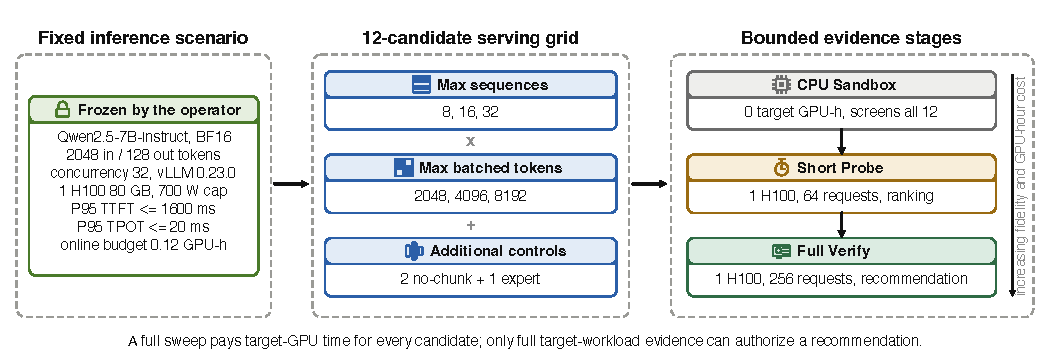
\includegraphics[width=\textwidth]{figures/results/fig1_decision_problem.pdf}
\caption{The bounded single-GPU decision problem.  A frozen model, workload,
SLO, and online budget define 12 immutable serving candidates: nine chunked
combinations from three sequence limits and three batched-token limits, two
no-chunk controls, and one expert default.  A full sweep pays target-GPU cost
for every candidate; \system{} instead screens all candidates in the CPU
Sandbox, escalates selected configurations to a short H100 Probe, and allows a
recommendation only after full target-workload verification.}
\label{fig:motivation}
\end{figure*}


\subsection{Observation 1: Configuration Rankings Are Conditional}

Prefill and decode stress different hardware resources, so a serving knob can
change energy and latency in opposite directions across token geometries.
Continuous batching, chunked prefill, prefix reuse, quantization,
and power policy further alter the realized schedule
\cite{kwon2023vllm,agrawal2024sarathi,zhong2024distserve,lee2026beam}.
Prior energy studies therefore find no universally best
model--engine--workload configuration
\cite{niu2025engines,fernandez2025energy}.  A useful search state must preserve
workload geometry, serving schedule, hardware state, and SLO, rather than reduce a
request to model FLOPs or mean GPU utilization.

\textbf{Requirement R1: scenario-conditioned decisions.}  The controller must
represent the complete deployment scenario and optimize the feasible frontier
for that intent, not learn one global configuration ranking.

\subsection{Observation 2: Cheap Evidence Is Useful but Not Authoritative}

Serving simulators can prune large configuration spaces after small profiling
campaigns \cite{agrawal2024vidur,yang2026charon}.  A single-GPU probe can also
measure prefill, decode, and power response directly.  Neither source observes
the full target run: the CPU model approximates runtime behavior, and a short
probe may not reach the target trace's batching, queueing, and thermal regime.
Prediction uncertainty must therefore grow when a candidate crosses an
unmeasured context, concurrency, serving-policy, or probe-duration boundary.

\textbf{Requirement R2: explicit evidence contracts.}  Every outcome must retain
its stage, provenance, and uncertainty.  A CPU estimate cannot be relabeled as
measured, a short probe cannot be relabeled as the target trace, and a released
recommendation must be supported by full target-workload evidence.

\subsection{Observation 3: Measurement Value Is Decision Dependent}

Uniform sweeps give equal priority to unequal decisions.  A candidate that is
clearly infeasible or dominated does not need a precise target-workload label.
By contrast, a cheap observation can be valuable when it changes the ordering
of two candidates near the frontier, resolves whether an SLO is met, or
calibrates a previously unseen workload or serving regime.  Generic predictive variance is also
insufficient: high uncertainty far from the feasible frontier may have no
effect on the final recommendation.

\textbf{Requirement R3: cost-normalized decision information.}  Acquisition
must jointly select configuration and fidelity according to expected change in
the high-fidelity SLO/Pareto decision per real GPU-hour.

\textbf{Requirement R4: bounded semantic autonomy.}  Natural-language intent,
heterogeneous execution failures, and human escalation benefit from an LLM
planner, but numerical prediction, feasibility, Pareto sorting, budget
accounting, and recommendation release must remain deterministic and auditable.
This separation makes the agent contribution testable against both an
optimizer-only controller and an LLM-only tool user.

\section{Problem Formulation}

An inference scenario is a tuple
\begin{equation}
S=\langle M,W,H,R,C,\mathbf o,B_m\rangle,
\end{equation}
where $M$ identifies the model and allowable precisions; $W$ is a request
trace or distribution over arrivals and token lengths; $H$ describes the
target GPU node and power controls; $R$ is the serving runtime; $C$ contains
memory, administrative, model-quality, and service-level constraints;
$\mathbf o$ specifies the objectives; and $B_m$ is the real-measurement budget
in GPU-hours.

The candidate space is
\begin{equation}
\mathcal X=\mathcal B\!\times\!\mathcal K\!\times\!\mathcal P\!\times\!
\mathcal F,
\end{equation}
covering sequence and batched-token budgets ($\mathcal B$), KV-cache policy
($\mathcal K$), prefill and batching policy ($\mathcal P$), and fixed or
tunable precision/power controls ($\mathcal F$).  A deterministic compiler
produces the scenario-feasible pool $\mathcal X_S$ by removing candidates that
violate memory capacity, runtime support, or site policy.

For $m$ objectives and evidence stages
$e\in\mathcal E=\{\textsc{Sandbox},\textsc{Probe},\textsc{Verify}\}$, let
$\mathbf f^{(e)}(x)\in\mathbb R^m$ denote the noisy response obtained by
querying candidate $x$ at stage $e$.  \textsc{Verify} executes the full target
workload on the target GPU and is the reference fidelity.  Our primary
minimization vector is
\begin{equation}
\mathbf f^{(v)}(x)=
\langle E_{\rm tok},T_{\rm TTFT},T_{\rm TPOT},-\Theta\rangle,
\end{equation}
where latency entries denote scenario-specified tail statistics and $\Theta$
is goodput or throughput.  If precision or model variants are part of the
search, their quality metric is enforced as a constraint rather than traded
silently for energy.  Let $q_S(x)=1$ when the verified response distribution
satisfies every service and quality constraint in $C$, and let
$\mathbf u\prec\mathbf v$ denote Pareto dominance under minimization.  The
unknown target set is
\begin{align}
\mathcal P_S^*=\{x\in\mathcal X_S:
&q_S(x)=1,\ \nexists x'\in\mathcal X_S\ \text{s.t.}\nonumber\\[-2pt]
&q_S(x')=1\land
\mathbf f^{(v)}(x')\prec\mathbf f^{(v)}(x)\}.
\label{eq:true-frontier}
\end{align}

At step $t$, the controller has evidence
$\mathcal D_t=\{(x_i,e_i,y_i,c_i,z_i)\}_{i=1}^t$, where $y_i$ is a
measured or simulated outcome, $c_i$ is realized GPU-hour cost, and $z_i$
records execution status and provenance.  An action $a_t=(x_t,e_t)$ yields an
observation and updates a belief over every verified response
$\mathbf f^{(v)}(x)$.  The returned set $\widehat{\mathcal P}_T$ contains only
fully verified candidates that satisfy the measured SLO and are nondominated
among the verified candidates; it is an estimate of, not an assumed subset
of, $\mathcal P_S^*$.

For a search policy $\pi$, we minimize a terminal decision loss
\begin{equation}
\min_{\pi}\
\mathbb E\!\left[\mathcal L
(\widehat{\mathcal P}_T,\mathcal P_S^*)\right]
\quad\text{s.t.}\quad
\sum_{t=1}^{T}c(a_t)\leq B_m,
\label{eq:budgeted-objective}
\end{equation}
where $\mathcal L$ combines normalized hypervolume regret with penalties for
false SLO feasibility and unverified release.  In bounded replay spaces we
compute $\mathcal P_S^*$ exhaustively; on live spaces we report verified
hypervolume, feasible precision/recall over the measured pool, and independent
holdout verification.  All search curves use cumulative real GPU-hours because
a CPU query, short probe, and full target run are not equivalent observations.

\section{\system{}\ Design}

\subsection{System Overview}

Figure~\ref{fig:architecture} shows the closed-loop, multi-fidelity Pareto
search and maps the requirements in Section~2 to concrete mechanisms.  The
Scenario Compiler enforces scenario conditioning (R1) by combining a typed
JSON/YAML specification with a natural-language intent and rejecting
infeasible candidates.  The evidence model and L0--L4 contracts preserve cross-scale
uncertainty (R2).  \ipig{}\ allocates measurement cost to decision-relevant
ambiguity (R3), while the guarded planner and Verifier bound semantic autonomy
(R4).  A language-model planner
observes the intent, a compact belief summary, remaining budget, failures, and
provenance, then emits one structured subgoal from \{\textsc{Explore},
\textsc{ResolveSLO}, \textsc{CalibrateScale}, \textsc{Repair}\}.  Final
\textsc{Verify} is entered only by the deterministic controller.  Within a
guarded search subgoal, \ipig{}\ selects the numerical
configuration--fidelity action.  The Tool Layer invokes serving simulation,
\bench{}\ templates, telemetry readers, and the scheduler.  Observations update
the Energy Twin and a versioned Evidence Store; the Verifier reruns final
Pareto candidates before scripts and recommendations are released.

\begin{figure*}[t]
\centering
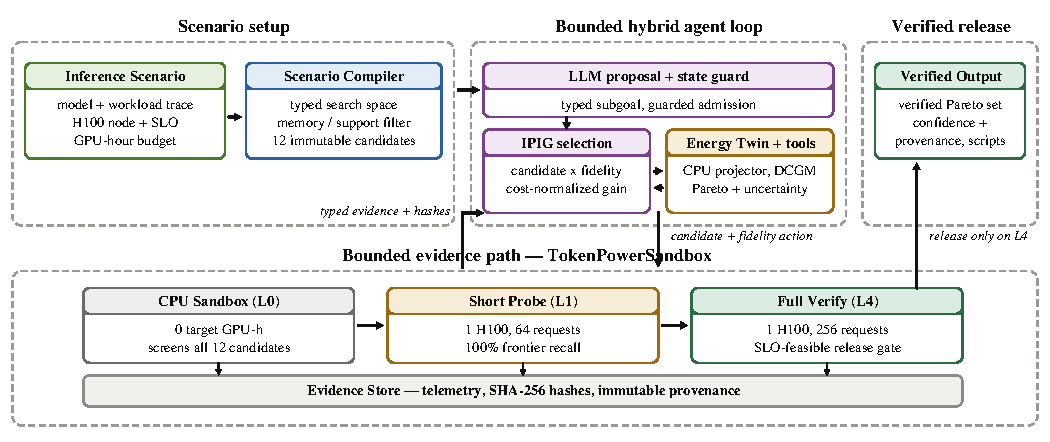
\includegraphics[width=\textwidth]{figures/results/fig2_system_overview.pdf}
\caption{\system{} overview.  The scenario compiler freezes a typed candidate
set and feasibility constraints.  The language model proposes an experiment
subgoal, the state guard admits or repairs it, and \ipig{} selects a
candidate--fidelity action.  The Energy Twin and deterministic tools produce
CPU predictions or measured H100 evidence, update uncertainty and the Pareto
set, and append telemetry and hashes to the evidence store.  Only full
target-workload Verify evidence can authorize the final recommendation.}
\label{fig:architecture}
\end{figure*}


\bench{}\ and \system{}\ consequently have separate responsibilities.  \bench{}\
defines and executes a measurement; \system{}\ decides which measurements are
decision-relevant, what can be inferred between them, and whether the evidence
supports a recommendation.  This separation also prevents circular claims:
the same simulator is never treated as ground truth for its own accuracy.

\subsection{Calibrated Energy Twin}

The implemented Energy Twin starts from a measured serving anchor and an
interpretable CPU projector.  It rejects memory-infeasible candidates, scales
prefill and decode work using token geometry and batch occupancy, predicts
active power between measured idle and active bounds, and preserves the
physical identity
\begin{equation}
\widehat E(W,x)=\widehat P(W,x)\widehat t(W,x).
\label{eq:energy-identity}
\end{equation}
For the present single-H100 study, one anchor cannot capture utilization
transitions across context length $L$ and concurrency $k$.  Relative to anchor
$(L_0,k_0)$, we therefore define
\begin{align}
q&=\log_2\!\frac{L_{in}+0.5L_{out}}{L_{in,0}+0.5L_{out,0}}, &
r&=\log_2\!\frac{k}{k_0},\\[-3pt]
\phi&=[q,r,qr,r^2].&&
\end{align}
For each directly predicted metric $m$, ridge regression fits
$\log(y_m/\widehat y_m^{base})=\beta_m^T\phi$.  Its strength is selected by
leave-one-workload-out error on a development split.  Throughput, power, TTFT,
and TPOT are corrected; energy is recomputed from corrected power and duration
rather than independently fitted.  Every calibration point retains repeat
dispersion and source hashes.

The topology projector additionally contains explicit TP/PP placement,
communication-volume, memory, and scale-distance terms.  At present these
terms produce machine-labeled extrapolations with enlarged uncertainty; they
are not publication-eligible multi-node predictions.  L2--L4 calibration on
H100/H200/B200 clusters is therefore an extension target rather than a claimed
result of this paper.

\subsection{Multi-Fidelity Sandbox Calibration}

The multi-fidelity sandbox is a bounded evidence environment implemented with
immutable job templates, container/runtime hashes, explicit resource
allocations, and fixed telemetry settings.  It does not pretend to reproduce a
large cluster on a laptop.  Instead, Figure~\ref{fig:calibration} organizes a
hierarchical set of evidence levels by the new effects they expose.

\begin{figure*}[t]
\centering
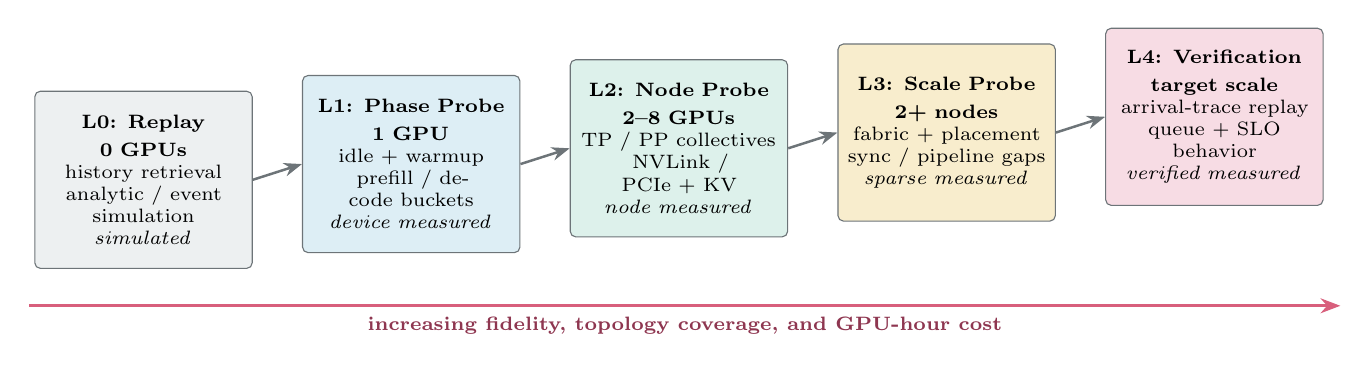
\begin{tikzpicture}[
  x=1cm,y=1cm,
  every node/.style={font=\sffamily},
  level/.style={draw=tpGray,rounded corners=2pt,minimum height=2.25cm,
    text width=2.55cm,align=center,inner sep=3pt,font=\scriptsize},
  flow/.style={-{Stealth[length=2.3mm]},line width=0.9pt,draw=tpGray}
]
  \node[level,fill=tpGrayLight] (l0) at (1.45,0.05)
    {\textbf{L0: Replay}\\[2pt]\textbf{0 GPUs}\\history retrieval\\analytic / event simulation\\\emph{simulated}};
  \node[level,fill=tpBlueLight] (l1) at (4.85,0.25)
    {\textbf{L1: Phase Probe}\\[2pt]\textbf{1 GPU}\\idle + warmup\\prefill / decode buckets\\\emph{device measured}};
  \node[level,fill=tpTealLight] (l2) at (8.25,0.45)
    {\textbf{L2: Node Probe}\\[2pt]\textbf{2--8 GPUs}\\TP / PP collectives\\NVLink / PCIe + KV\\\emph{node measured}};
  \node[level,fill=tpGoldLight] (l3) at (11.65,0.65)
    {\textbf{L3: Scale Probe}\\[2pt]\textbf{2+ nodes}\\fabric + placement\\sync / pipeline gaps\\\emph{sparse measured}};
  \node[level,fill=tpRoseLight] (l4) at (15.05,0.85)
    {\textbf{L4: Verification}\\[2pt]\textbf{target scale}\\arrival-trace replay\\queue + SLO behavior\\\emph{verified measured}};

  \draw[flow] (l0.east) -- (l1.west);
  \draw[flow] (l1.east) -- (l2.west);
  \draw[flow] (l2.east) -- (l3.west);
  \draw[flow] (l3.east) -- (l4.west);
  \draw[-{Stealth[length=2.5mm]},very thick,tpRose]
    (0.0,-1.55) -- node[below,font=\scriptsize\bfseries,text=tpRoseDark]
    {increasing fidelity, topology coverage, and GPU-hour cost} (16.65,-1.55);
\end{tikzpicture}
\caption{Multi-fidelity sandbox calibration.  Each hierarchical level exposes
effects that cannot be inferred reliably below it.  The agent escalates only
candidates whose uncertainty can change SLO feasibility or the Pareto frontier;
a final deployment recommendation requires target-scale trace verification.}
\label{fig:calibration}
\end{figure*}


\begin{itemize}
    \item \textbf{L0 -- replay/simulate (0 GPUs):} retrieve nearby \bench{}\
    records and run analytic or discrete-event simulation.
    \item \textbf{L1 -- phase probes (1 GPU):} measure idle/warmup, length- and
    batch-bucketed prefill, controlled decode, and power-policy response.
    \item \textbf{L2 -- intra-node probes (2--8 GPUs):} calibrate TP/PP,
    collective volume, NVLink/NVSwitch or PCIe behavior, and KV-cache pressure.
    \item \textbf{L3 -- sparse multi-node probes (2+ nodes):} sample selected
    scale points to expose fabric, synchronization, placement, and pipeline
    effects.  This level is deliberately sparse and chosen actively.
    \item \textbf{L4 -- target-trace verification:} replay the intended request
    trace for the top-$k$ configurations at target scale and report the result
    as measured evidence.
\end{itemize}

Levels are scenario-relative.  In the present single-H100 search, L1 is a
64-request probe and L4 is the full 256-request target workload on the same GPU;
L2 and L3 are skipped because the scenario contains no intra- or inter-node
scale transition.  A future multi-node scenario would activate those levels
without changing the controller or evidence schema.

A result carries its highest supporting level.  L0 outputs are
\emph{simulated}; predictions between observed settings are \emph{interpolated};
cross-topology predictions are \emph{extrapolated}; and only L1--L4 telemetry
is \emph{measured}.  This vocabulary is encoded in the artifact schema and
used in every table and plot.

\subsection{Hybrid Belief-State Policy and \ipig{}}

The controller observes predictive uncertainty, Pareto ambiguity, distance to
an SLO boundary, topology novelty, remaining budget, and run failures within
the loop in Figure~\ref{fig:architecture}.  It rejects invalid candidates
deterministically.  For each $x$, define high-fidelity feasibility and Pareto
membership variables $Q_x=\mathbf 1[q_S(x)=1]$ and
$P_x=\mathbf 1[x\in\mathcal P_S^*]$.  The intent-specific terminal decision is
\begin{equation}
\Omega_S=\{(Q_x,P_x):x\in\mathcal X_S\}.
\end{equation}
For an admissible action $a=(x,\ell)$, the policy interface targets
\begin{equation}
\alpha_t(a\mid S)=
\frac{I(Y_a;\Omega_S\mid\mathcal D_t,S)}
{(\mathbb E[c(a)\mid\mathcal D_t]+\epsilon)^\gamma}.
\label{eq:ipig}
\end{equation}
The numerator denotes information about the L4 SLO-feasible Pareto decision,
not generic prediction variance.  The current artifact exposes this estimator
as a typed interface and uses a transparent proxy
\begin{equation}
\widetilde I_t(a)=U_t(x)
\left(.45p_{P}(x)+.35p_{S}(x)+.20d_{T}(x)\right)g_\ell,
\label{eq:ipig-proxy}
\end{equation}
where $U_t$ is predictive uncertainty, $p_P$ approximates frontier relevance,
$p_S$ approximates proximity to an SLO boundary, $d_T$ flags unresolved
topology transfer, and $g_\ell$ is a monotone fidelity gain.  The semantic
subgoal increases the corresponding SLO or topology term.  The score divides
Eq.~\ref{eq:ipig-proxy} by declared GPU cost as in
Eq.~\ref{eq:ipig}; actions that exceed the remaining exploration budget are
removed first.  This proxy is auditable and sufficient for the Workshop
agent-loop study.  Replacing it with nested-posterior Pareto mutual information
is reserved for the larger MLSys evaluation.

The semantic subgoal restricts the admissible actions before maximizing
Eq.~\ref{eq:ipig}.  \textsc{ResolveSLO} admits candidates whose intervals
cross an SLO; \textsc{CalibrateScale} requires topology-sensitive features;
and the deterministic \textsc{Verify} state admits only L4 actions.
Operationally, the resulting
states are:
\begin{itemize}
    \item \textbf{Simulate} when the candidate is in-domain and its confidence
    interval cannot alter the feasible frontier.
    \item \textbf{Calibrate} when a local measurement can change ranking,
    reduce topology uncertainty, or resolve an SLO boundary.
    \item \textbf{Verify} when a candidate will be recommended, when scale
    extrapolation remains material, or when independent evidence is required.
\end{itemize}
Exploratory search terminates when its budget is exhausted or the probability
of a frontier change falls below a threshold.  A reserved verification budget
then supports L4 runs for the top-$k$ candidates; no recommendation is released
without target-scale evidence.

\subsection{Bounded Autonomy and Provenance}

The LLM can choose from typed tools but cannot issue an unrestricted shell
command, modify model weights, change telemetry intervals, or enlarge a Slurm
allocation without approval.  Numeric calculations, feasibility, Pareto
sorting, and budget accounting are deterministic.  Every action records the
scenario and configuration hashes, prompt and tool versions, evidence level,
job ID, raw-data URI, simulator checkpoint, uncertainty, and decision rationale.
The Verifier checks units, missing samples, clock/power state, run completion,
and agreement between GPU and node telemetry before accepting evidence.

\section{Reference Implementation}

\subsection{Scenario and Evidence Interfaces}

The prototype accepts a versioned JSON or YAML scenario containing model,
workload, target GPU, objectives, SLO, candidate serving knobs, available
evidence stages, stage costs, and verification budget.  The compiler expands
knob lists into immutable candidates and checks resource requirements before
search.  Each evidence record stores scenario/candidate hashes, realized token
histograms, software versions, GPU identity, phase timestamps, power streams,
latency/goodput, evidence stage, status, and raw-data checksum.  Existing
\bench{} records are imported read-only; new jobs use the same configuration
vocabulary.

\subsection{Implemented Evidence Path}

The Probe/Verify path uses a digest-pinned vLLM server and a read-only client on
an internal Docker network.  Workload-transfer trials keep the server
persistent; configuration campaigns restart it from a pinned template when
knobs change.  The path disables prefix caching, fixes temperature at zero, and
ignores EOS.  A two-FIFO \texttt{READY/GO/DONE/ACK} handshake places host-side
reads of DCGM's cumulative device-energy counter around the main benchmark
interval, excluding loading, health checks, warmups, and result formatting.
The calibration builder aggregates compatible Probe repeats by their median
and records dispersion and source SHA-256.  The CPU Sandbox retains uncertainty
and scope labels; freeze and validation tools reject modified or late
predictions, mismatched repeats, and split leakage.

\subsection{Component Architecture and Status}

Five typed boundaries expose the \textbf{scenario compiler}, \textbf{history
retrieval}, \textbf{Energy Twin}, \textbf{executor}, and
\textbf{planner/policy}.  CPU prediction, replay, Probe/Verify serving
execution, balanced configuration campaigns, evidence freezing, blind
validation, corpus construction, and policy benchmarking are implemented.  The
constrained planner calls an OpenAI-compatible endpoint, accepts only a JSON
subgoal and rationale, and falls back to the deterministic planner on malformed
output or endpoint failure.  Candidate selection and every safety-critical
state transition remain outside the language model.

All executors share a typed interface keyed by candidate, evidence stage, and
seed.  Replay returns a hidden sealed row only after an action requests it; the
CPU Sandbox returns a scoped prediction; and the serving executor performs the
short Probe or full Verify run.  All three return the same evidence object, so
the planner, guard, policy, and belief update remain backend-independent.

\subsection{Closed-Loop Search}

Algorithm~\ref{alg:search} specifies the implemented controller.  It reserves
top-$k$ Verify cost, then chooses a candidate--stage action whose uncertainty
can change feasibility or dominance.  Failed jobs consume budget and update the
evidence state rather than disappearing from analysis.  Every event stores
uncertainty and predicted-frontier snapshots before and after observation,
cumulative and remaining GPU-hours, evidence kind, planner source, and any
fallback reason.

\begin{algorithm}[t]
\caption{Evidence-gated single-GPU Pareto search}
\label{alg:search}
\footnotesize
\begin{algorithmic}[1]
\REQUIRE scenario $S$, history $\mathcal D_0$, budget $B_m$, verify count $k$
\STATE $\mathcal X\gets\textsc{CompileAndValidate}(S)$
\STATE $\mathcal D\gets\mathcal D_0$; $\mathcal T\gets\textsc{FitTwin}(\mathcal D_0,S)$
\STATE $(B_s,B_v)\gets\textsc{ReserveVerification}(B_m,S,k)$
\WHILE{$B_s>0$}
  \STATE $g_t\gets\textsc{SemanticPlan}(S,\mathcal T,\mathcal D,B_s)$
  \STATE $\mathcal A_s\gets\textsc{GuardAvailableStages}(g_t,\mathcal X,B_s)$
  \STATE $(x^*,e^*)\gets\arg\max_{(x,e)\in\mathcal A_s}
  \alpha_t((x,e)\mid S)$
  \IF{$\alpha_t(x^*,e^*)<\tau_A$ or frontier stable for $p$ steps}
    \STATE \textbf{break}
  \ENDIF
  \STATE $y\gets\textsc{AcquireEvidence}(x^*,e^*)$
  \STATE $\mathcal D\gets\mathcal D\cup\{y\}$; $B_s\gets B_s-c(x^*,e^*)$
  \STATE $\mathcal T\gets\textsc{UpdateTwin}(\mathcal T,y)$
\ENDWHILE
\STATE $(\hat{\mathbf f},\mathbf U)\gets\textsc{Predict}(\mathcal T,\mathcal X)$
\STATE $\hat{\mathcal P}\gets\textsc{SLOFeasiblePareto}(\hat{\mathbf f},\mathbf U)$
\STATE $\mathcal P_v\gets\textsc{VerifyTopK}(\hat{\mathcal P},S,k,B_v)$
\STATE \textbf{return} $\mathcal P_v$, provenance, and runnable scripts
\end{algorithmic}
\end{algorithm}

\subsection{Execution Isolation and Failure Handling}

The measurement controller changes one frozen serving template at a time,
waits for a health check, performs an unmeasured warmup, and then opens the
energy boundary.  The client has no external network route, the container is
read-only apart from bounded temporary storage, and every configuration restart
is logged.  The executor distinguishes launch failure, timeout, out-of-memory,
telemetry loss, malformed output, and SLO failure.  Recoverable failures can be
retried from the deterministic template; configuration changes create a new
hash and evidence record.  A failed action is charged its declared upper-bound
cost and can trigger \textsc{Repair}, but it cannot be removed from accounting.

\section{Evaluation Methodology}

The Workshop evaluation separates two questions that are often conflated.
First, is the cheap evidence consumed by the agent accurate and calibrated
enough to support a decision?  Second, given a sealed candidate corpus, does
the acquisition policy spend fewer GPU-hours reaching a verified decision?
Simulation never defines its own ground truth.

\subsection{Research Questions}

\textbf{RQ1 -- Evidence validity.}  How accurately does the CPU-first model
rank and predict unseen H100 energy, throughput, TTFT, and TPOT as context
length and concurrency change?

\textbf{RQ2 -- Scope reliability.}  Can a preregistered release rule identify
where predictions are reliable and abstain where performance fidelity does not
transfer?

\textbf{RQ3 -- Search efficiency.}  On a frozen serving-configuration corpus,
how much Pareto quality does the IPIG proxy recover per GPU-hour relative to
random, cost-blind information gain, and a fixed cheapest-first ladder?

\textbf{RQ4 -- Bounded autonomy.}  Does the runtime enforce budgets, preserve
evidence labels, recover from tool failures, reject malformed planner output,
and withhold every recommendation lacking L4 verification?

\subsection{H100 Evidence Study}

Experiments use one H100 80GB at a 700-W power limit and
Qwen2.5-7B-Instruct with a digest-pinned vLLM 0.23.0 image.  The fixed serving
configuration is BF16, TP$=$PP$=$DP$=$1, 256 maximum sequences, 8192 batched
tokens, chunked prefill, and no prefix caching.  Requests use fixed output
length, temperature zero, and ignore EOS.  A cumulative DCGM device-energy
counter brackets only the active benchmark window; loading, health checks,
graph capture, and warmup are excluded.  Every point has three repeats and is
summarized by median and MAD.

Three anchor repeats use 512 input and 128 output tokens at concurrency eight.
A six-workload development split selects the residual correction by
leave-one-workload-out error.  Predictions and their SHA-256 manifest are then
frozen before each holdout begins.  The first holdout contains eight workloads
and \HoldoutMeasurements{} measurements spanning 256--2048 input tokens and
concurrency 1--32.  Without refitting, a second preregistered confirmation
contains nine workloads and \ConfirmationMeasurements{} measurements at
contexts 384, 768, and 1536 and concurrency 1, 2, and 4.  The validator checks
prediction time, dataset split, workload, configuration, power limit, repeat
identity, and all raw-artifact hashes.

Primary evidence metrics are energy MAPE, Spearman rank correlation, pairwise
ordering accuracy, and repeat CV.  Throughput, TTFT, and TPOT are secondary
endpoints.  Before confirmation, we preregister energy MAPE $\leq15\%$ over
all nine workloads and TTFT MAPE $\leq20\%$ at concurrency four.  If TTFT MAPE
exceeds 20\% below concurrency four, the released scope must abstain there.

\subsection{Agent Replay Protocol}

The agent study varies serving configurations while holding a workload fixed.
A bounded H100 grid changes maximum sequences, maximum batched tokens, and
chunked prefill after deterministic memory guards.  Each feasible candidate is
measured three times in randomized order, and all L0 predictions are frozen
before the first L1 run.  Successful highest-fidelity records define the
SLO-feasible oracle frontier using median metrics.

Each policy starts from identical priors and a reserved L4 verification budget.
It sees a row only after requesting its candidate--fidelity pair.  We run
\AgentEpisodes{} seeded episodes for IPIG, random acquisition, cost-blind
information gain, and a cheapest-first ladder.  Random and cheapest-first do
not receive the semantic action guard.  Reported metrics are verified Pareto
precision/recall, primary-objective regret, GPU-hours to the first oracle hit,
total GPU-hours, failed actions, and unnecessary L4 escalations.  Replay seeds
bind each candidate--fidelity pair to the same replicate across policies.  The
runner constructs the oracle only from sealed measured records and embeds the
scenario and corpus hashes in its report.

\subsection{Reliability Tests}

Unit and end-to-end tests inject missing evidence, malformed LLM JSON, launch
failure, an exhausted budget, and an SLO-violating verification.  A failed job
is charged its declared upper-bound cost and becomes an immutable failed
record; it cannot disappear from accounting.  The next planner state exposes
the failure and enters \textsc{Repair}.  The LLM selects only a semantic
subgoal, while candidate choice, command routing, budget arithmetic, Pareto
filtering, and the final L4 gate remain deterministic.

\section{Results}

\subsection{RQ1: Cheap Evidence Preserves Energy Decisions}

Table~\ref{tab:evidence-results} summarizes the two sealed holdouts.  On the
eight-workload v2 holdout, energy MAPE is \CalibratedEnergyMAPE{}, median APE is
\EnergyMedianAPE{}, and the maximum APE is \EnergyMaxAPE{}.  Energy rank
correlation is \EnergySpearman{}, and \EnergyPairwise{} pairwise orderings
(\EnergyPairwisePct{}) are correct.  Median repeat CV is only
\EnergyRepeatCV{}, indicating that prediction error, rather than measurement
noise, dominates.  Throughput and TPOT MAPE are
\CalibratedThroughputMAPE{} and \CalibratedTPOTMAPE{}.  TTFT is less accurate
at \CalibratedTTFTMAPE{}, motivating the separate release gate below.

Without refitting, scope confirmation obtains \ConfirmationEnergyMAPE{}
energy MAPE, \ConfirmationEnergySpearman{} rank correlation, and
\ConfirmationEnergyPairwise{} correct pairwise orderings.  Its largest energy
error is \ConfirmationEnergyMaxAPE{}, so the preregistered 15\% primary
endpoint passes on all nine workloads.  The result supports CPU-first energy
screening inside the measured workload and runtime envelope; it does not
establish cross-GPU or multi-node accuracy.

\begin{table}[t]
\centering
\caption{Frozen-model results on two disjoint H100 holdouts.  Each workload
has three repeats; MAPE compares the frozen prediction with the observed
median.}
\label{tab:evidence-results}
\small
\setlength{\tabcolsep}{3.8pt}
\begin{tabular}{lrrrr}
\toprule
Study & Workloads & Runs & Energy MAPE & $\rho$ \\
\midrule
Holdout v2 & \HoldoutWorkloads{} & \HoldoutMeasurements{} &
\CalibratedEnergyMAPE{} & \EnergySpearman{} \\
Scope v3 & \ConfirmationWorkloads{} & \ConfirmationMeasurements{} &
\ConfirmationEnergyMAPE{} & \ConfirmationEnergySpearman{} \\
\bottomrule
\end{tabular}
\end{table}


\subsection{RQ2: Scope Gating Prevents a False Latency Claim}

Aggregate TTFT MAPE in the confirmation is \ConfirmationTTFTMAPE{}, which by
itself would reject a global TTFT claim.  Stratification reveals the boundary
in Table~\ref{tab:scope-results}.  At concurrency four, TTFT MAPE is
\KFourTTFTMAPE{} and maximum APE is \SupportedTTFTMaxAPE{}, passing the
preregistered 20\% rule.  At concurrency one and two, TTFT MAPE rises to
\KOneTTFTMAPE{} and \KTwoTTFTMAPE{}; the combined sparse-stratum error is
\SparseTTFTMAPE{}.  The generated decision therefore supports latency at
concurrency at least four and abstains below four.  Energy remains stable in
all three strata.  This is the desired behavior for an evidence-gated agent:
it narrows a claim instead of turning confident energy estimates into an
unsupported latency recommendation.

\begin{table}[t]
\centering
\caption{Preregistered scope-confirmation MAPE by concurrency.}
\label{tab:scope-results}
\small
\setlength{\tabcolsep}{4.2pt}
\begin{tabular}{crrrr}
\toprule
Conc. & Energy & Throughput & TPOT & TTFT \\
\midrule
1 & \KOneEnergyMAPE{} & \KOneThroughputMAPE{} &
\KOneTPOTMAPE{} & \KOneTTFTMAPE{} \\
2 & \KTwoEnergyMAPE{} & \KTwoThroughputMAPE{} &
\KTwoTPOTMAPE{} & \KTwoTTFTMAPE{} \\
4 & \KFourEnergyMAPE{} & \KFourThroughputMAPE{} &
\KFourTPOTMAPE{} & \KFourTTFTMAPE{} \\
\bottomrule
\end{tabular}
\end{table}


\subsection{RQ3: Configuration-Search Efficiency}

The runtime can already execute sealed replay episodes for IPIG, random,
cost-blind, and cheapest-first policies and produce all metrics in
Table~\ref{tab:agent-results}.  The bundled three-candidate corpus is explicitly
synthetic and is used only for software tests.  Publication values require the
frozen H100 serving-configuration corpus described in Section~VII; until that
campaign is sealed, we make no claim that IPIG outperforms a search baseline.

\begin{table}[t]
\centering
\caption{Sealed controller results.  Policy rows use
\BudgetEpisodesPerPoint{} matched episodes/budget; AUC spans \BudgetLevels{}
budgets.  Planner rows use \PlannerCallsPerSet{} calls/set; V2 is a disjoint
holdout.  Guard event is V1 fallback or V2 intervention; latency is P50/P95 ms.}
\label{tab:agent-results}
\footnotesize
\setlength{\tabcolsep}{3.0pt}
\textbf{(a) Acquisition policy}\par\vspace{2pt}
\begin{tabular}{lrrr}
\toprule
Policy & Hit@.12 & Mean GPU-h & Success AUC \\
\midrule
\ipig{} & \IPIGOracleHit{} & \IPIGGPUHours{} & \IPIGSuccessAUC{} \\
Random & \RandomOracleHit{} & \RandomGPUHours{} & \RandomSuccessAUC{} \\
Cost-blind & \CostBlindOracleHit{} & \CostBlindGPUHours{} & \CostBlindSuccessAUC{} \\
Cheapest-first & \CheapestOracleHit{} & \CheapestGPUHours{} & \CheapestSuccessAUC{} \\
\bottomrule
\end{tabular}
\par\vspace{2pt}
\textbf{(b) Semantic planner}\par\vspace{2pt}
\begin{tabular}{lrrrr}
\toprule
Set & Raw & Admitted & Guard event & P50/P95 \\
\midrule
V1 development & \PlannerVoneRaw{} & \PlannerVoneAdmitted{} &
\PlannerVoneFallback{} & \PlannerVoneMedianLatency{}/\PlannerVonePninetyfiveLatency{} \\
V2 holdout & \PlannerVtwoRaw{} & \PlannerVtwoAdmitted{} &
\PlannerVtwoIntervention{} & \PlannerVtwoMedianLatency{}/\PlannerVtwoPninetyfiveLatency{} \\
\bottomrule
\end{tabular}
\end{table}


\subsection{RQ4: Bounded Runtime Behavior}

All 58 automated tests pass.  Injected executor failure becomes a failed
evidence record charged at its declared cost, and the next event enters
\textsc{Repair}.  Malformed LLM output triggers a recorded rule-based fallback.
Replay and topology tools cannot relabel L0/L2 outputs as verified, budget
overruns raise a hard error, and the returned recommendation set is computed
only from successful L4 evidence that satisfies the SLO.  These tests establish
mechanism enforcement, not the semantic quality of a particular planner model.

\section{Related Work}

\subsection{Energy Measurement, Serving, and Simulation}

Inference-energy studies establish joules/token and joules/request as
first-class metrics and show sensitivity to model, workload, hardware, engine,
decoding, and parallelism
\cite{samsi2023words,fernandez2025energy,niu2025engines}.  MLPerf Power,
and \bench{} add cross-scale measurement and declarative phase-aligned GPU,
component, and node telemetry \cite{tschand2024mlperf,niu2026tokenpowerbench}.
They supply observations but do not allocate a scenario-specific budget for
the next observation.

Serving systems expose the knob space through memory management, chunked
prefill, and disaggregation \cite{kwon2023vllm,agrawal2024sarathi,
zhong2024distserve}.  Vidur uses profiling for what-if analysis, Charon combines
profiled and analytical operator backends, and Meta searches millions of
deployment configurations \cite{agrawal2024vidur,yang2026charon,
cho2026deployment}.  These works establish strong simulator priors;
\system{} asks when a prior is sufficient and when measurement is worth its
cost.

\subsection{Energy Control and Multi-Fidelity Optimization}

DynamoLLM and GreenLLM optimize cluster size, parallelism, or frequency under
SLOs \cite{stojkovic2024dynamollm,liu2025greenllm}.  BEAM jointly controls GPU
frequency, prefill chunks, and microbatches using an offline energy--performance
table \cite{lee2026beam}; BOute applies constrained qNEHVI to deployment Pareto
search, and OptiKIT uses full H100 trials for SLO-driven serving tuning
\cite{jiang2026boute,santavas2026optikit}.  They optimize deployment or runtime
actions under a fixed observation model.  \system{} instead optimizes the
evidence-acquisition process before a verified recommendation.

Generic multi-fidelity Pareto optimization is the closest algorithmic
precedent.  MF-OSEMO selects candidate--fidelity vectors using highest-fidelity
frontier information, while MF-JESMOC adds constraints
\cite{belakaria2020mfosemo,fernandezsanchez2025mfjesmoc}.  We do not claim the
first information-gain optimizer.  \ipig{} conditions the terminal variable on
intent-specific SLO feasibility and Pareto membership, then adds typed evidence,
guarded execution, and mandatory verified release.

\subsection{Agentic Systems Optimization}

ReAct separates language reasoning from external actions \cite{yao2023react}.
STELLAR tunes parallel file systems, and PROMPTS uses profiler feedback for
multi-agent configuration recommendation
\cite{egersdoerfer2025stellar,ding2026prompts}.  AIOpsLab shows
that operational agents need controlled workloads, telemetry, fault injection,
and outcome-based evaluation \cite{chen2025aiopslab}.  We test a narrower
architectural question: can semantic proposals be evaluated and admitted
safely while numerical evidence selection remains auditable?  Raw planner
agreement and guarded decisions are therefore reported separately; we do not
attribute the guard's correctness to the language model.

Across these areas, the joint gap is configuration--fidelity co-selection under
real GPU-hour cost followed by full target-workload verification.  No individual
component is claimed as novel in isolation.

\section{Artifact and Reproducibility}

The artifact contains versioned scenarios, grids, evidence schemas, CPU,
replay, and serving executors, the bounded controller, four policies,
calibration/validation tools, and \AutomatedTests{} tests.  Each event records
the proposed and admitted subgoal, guard action, candidate, fidelity, cost,
uncertainty, Pareto state, budget, evidence kind, metrics, and fallback.

H100 evidence bundles preserve raw 100-ms telemetry, benchmark output, frozen
predictions and schedules, reports, and nested SHA-256 manifests.  The
configuration bundle verifies \ConfigurationRawArtifacts{} raw entries and an
\ConfigurationReplayRows{}-row corpus; the paired follow-up likewise hashes its
freeze, \WinnerConfirmationRuns{} measurements, and raw outputs.  Predictions
precede measurements, raw evidence precedes analysis, and confirmation permits
neither refitting nor reselection.

Replay reveals rows only when their candidate--stage keys are requested and
forms the oracle from successful Verify metrics.  An early aliased report is
archived but excluded; commit \texttt{c41d8a6} supplies action-specific common
random numbers.  Archived JSON keeps legacy \texttt{level} tags
\texttt{L0/L1/L4} for compatibility; these are provenance identifiers, not
stages.  We use Sandbox, Probe, and Verify throughout.

The artifact also freezes the five-budget study and both planner protocols,
including prompts, states, raw responses, decisions, latency, and guard
interventions.  Disjoint V1/V2 identifiers preserve V2's failed raw gate;
compact summaries accompany SHA-256-identified raw archives.

\section{Limitations and Threats to Validity}

\textbf{Empirical scope.}  The study deliberately covers one H100, one 7B
model, one vLLM version, BF16, fixed output length, and bounded
workload/configuration grids.  The measured knob search varies sequence and
token limits plus chunked prefill.  The claims are therefore about evidence
allocation on one target GPU, not parallel or distributed serving.

\textbf{Fidelity and telemetry.}  DCGM cumulative energy captures GPU-device
rather than host or facility energy.  The CPU Sandbox and short Probe may both
miss behavior outside the frozen model, software, workload, and hardware scope;
the Sandbox TTFT inversion observed here further shows that good energy ranking
must not be generalized to every metric.  TP/PP, cross-hardware, MoE, and
multi-node communication require new measured calibration and verification and
are reserved for a broader follow-on study.

\textbf{Uncertainty and policy value.}  Prediction intervals are not calibrated
across hardware generations; new kernels, engines, GPUs, arrival processes, or
MoE routing may invalidate residual corrections.  The current \ipig{} estimator
is an auditable proxy rather than exact Pareto mutual information.  Its
\PolicyEpisodes{} episodes per policy bootstrap only \PolicyHardwareRepeats{}
real repeats per candidate--stage key, so they measure sensitivity to observed
run-to-run variation rather than independent production deployments.  \ipig{}
beats random and cost-blind acquisition on the declared cost--success metrics
but not cheapest-first in this small grid.  The exhaustive
\ConfigurationTotalGPUHours{}-GPU-h corpus validates fidelity and supplies an
oracle; replay does not erase that offline data-collection cost.

\section{Conclusion}

\system{} turns energy-aware LLM inference tuning into a bounded
evidence-allocation loop: interpret intent, choose a configuration and
fidelity, observe immutable evidence, update an SLO-feasible Pareto belief, and
verify before recommending.  Its deterministic guard keeps the LLM away from
commands, budgets, numeric optimization, and release authority.  On
\BlindMeasurements{} blind H100 measurements, the underlying CPU-first model
achieves \CalibratedEnergyMAPE{} and \ConfirmationEnergyMAPE{} energy MAPE in
two disjoint holdouts.  The preregistered gate also exposes a meaningful
boundary: TTFT transfers at concurrency four but requires abstention below
four.  These results establish a trustworthy evidence substrate and an
implemented agent runtime.  The immediate remaining experiment is to quantify
Pareto quality per GPU-hour on a frozen serving-configuration corpus; broader
H100/H200/B200 and multi-node optimization is reserved for the MLSys study.


\balance
\bibliographystyle{IEEEtran}
\bibliography{references}

\end{document}
